\documentclass[parskip=full, numbers=noenddot]{scrreprt}

\usepackage[english]{babel}
\usepackage[utf8]{inputenc}
\usepackage{csquotes}
\usepackage[
  backend=biber,
  doi=false,
  isbn=false,
  url=false,
  date=year,
  style=alphabetic,
  citestyle=authoryear]{biblatex}
\addbibresource{dissertation.bib}

\usepackage{graphicx}
  \graphicspath{ {./graphics/} }
\usepackage{subcaption}
\usepackage{url}
\usepackage{varioref}
\usepackage{tabularx}
  \newcolumntype{L}{>{\raggedright\arraybackslash}X}
\usepackage[version=4]{mhchem}
\usepackage{siunitx}
\DeclareSIUnit\molar{\mole\per\cubic\deci\metre}
\DeclareSIUnit\Molar{\textsc{m}}
\usepackage{booktabs}
\usepackage{longtable}

\title{Quantifying the bias in SELEX procedure}
\author{Candidate number XXXXX}

\begin{document}

\maketitle
% Will deal with the intricacies of the cover pages at the very end.

\begin{abstract}
 
Summary.
 
\end{abstract}

\tableofcontents

\chapter*{List of Abbreviations}
\label{ch:abbrev}

List of Abbreviations.

\chapter{EMSA-SELEX}
\label{ch:emsaselex}

\section{Introduction}
\label{sec:emsaselex_intro}

\subsection{Physiological importance of the nucleosome, nucleosome occupancy, and gene expression}
\label{ssec:emsaselex_intro_importance}

%% Physiological importance of the nucleosome

% CDB notes will help. Treat this as an essay...?
Eukaryotes package their DNA into chromatin through a series of coiling steps.  The fundamental repeating unit of chromatin is the nucleosome.  The nucleosome consists of a histone octamer with 147 base pairs (bp) of DNA wrapped around it.  Apart from roles in supercoiling, nucleosomes inhibit binding of DNA-binding proteins to DNA.  Therefore placement of nucleosomes at favoured positions in the genome affects gene expression.  Wherever nucleosomes are, transcription is inhibited as RNA polymerases cannot bind to DNA.  Activation of this transcription is changed because activators and repressors cannot bind to \emph{cis}-regulatory elements.
% Epigenetics: how relevant is this? how cohesive is this to the rest of this section?
Epigenetics extends on these principles.  Chemical modifications to histone octamers in nucleosomes affect the degree of chromatin packing, and therefore accessibility of chromatin to DNA-binding proteins and transcription factors.

%% Nucleosome occupancy

Nucleosome positioning defines where nucleosomes are positioned within the genome(\cite{struhl_determinants_2013}).
In contrast, nucleosome occupancy refers to the proportion of cells in a population that have a histone at a specific region in the genome. % Struhl and Segal, 2013.
Because nucleosomes inhibit binding of DNA-binding proteins to DNA, nucleosome positioning and nucleosome occupancy are important determinants in gene expression. % is this redundant?

\subsection{Nucleosome sequence preferences}
\label{ssec:emsaselex_intro_seqpref}
% - Previous researches on nucleosome’s sequence preferences

The nucleotide sequence in DNA contributes to nucleosome positioning.  For a given 147-bp DNA sequence, the affinity of the histone octamer can vary over more than three orders of magnitude.

Nucleotide sequences affect flexibility of the DNA around histone octamers.  The dinucleotide sequences AA, AT, and TA confer high `bendability' to DNA.  Therefore, they are situated on the face of the helical repeat that directly interacts with the histone octamer, with a periodicity of approximately 10 bp.  GC dinucleotides also occur periodically, but out of phase with the aforementioned dinucleotides.  These preferences were confirmed by a computational model of nucleosome-DNA interaction, which includes a based on a position-weight matrix to score any 147-bp nucleotide sequence for the probability that it is associated with a nucleosome, employing dinucleotide probability distributions.  The data was based on yeast-based genome-wide assay that identified DNA regions that were stably wrapped in nucleosomes \cite{segal_genomic_2006}.

In contrast, the homopolymeric sequences poly(dA:dT) and poly(dG:dC) confer stiff structures that inhibit nucleosome formation.  These sequences are therefore enriched in linker DNA between nucelosomes.  Poly(dA:dT) sequences are enriched in promoters, in particular that of \emph{Saccharomyces cerevisiae}.  Depletion of nucleosomes at promoters on artificial chromosomes based on \emph{S. cerevisiae} genomic regions was shown to be dependent on the number and length of poly(dA:dT) sequences (\cite{hughes_functional_2012}), supporting this.
% move this to `gene expression'?
With these properties, evolution has altered poly(dA:dT) tracts to fine-tune gene expression in organisms. % unclear

\cite{segal_genomic_2006} also show that there is low nucleosome occupancy at functional binding sites.  This is based on how binding sites for 37\% of transcription factors investigated have lower nucleosome occupancy than predicted.  It was also shown that there is low nucleosome occupancy at transcription start sites.  \cite{huff_dnmt1-independent_2014} show that nucleosomes are positioned downstream of transcription start sites in algae despite high GC content by using micrococcal nuclease digestion assays.


DNA methylation also affects nucleosome positioning.
% Dnmt1-indepedent CG methylation contributes to nucleosome positioning in diverse eukaryotes (Huff and Zilberman, 2014)
% this is from the intro of Huff and Zilberman
However, studies conflict on whether DNA methylation is positively correlated or negatively correlated with nucleosome presence.  Several studies suggest that methylation preferentially occurs outside or at the edges of nucleosome cores, while one study shows that methylation is enriched in the nucleosome core. % citations needed
% this is from experiments by Huff and Zilberman
Methylation of DNA in the algae \emph{Ostreococcus lucimarinus} and \emph{Micromonas pusilla} occurs in the linker DNA between nucleosome, and is almost completely excluded from nucleosome cores.  This is based on micrococcal nuclease digestion.  


% Genome-wide mapping of nucleosome positioning and DNA methylation within individual DNA molecules (Kelly et al, 2012)

Importantly, these models of nucleosome positioning are based on studies that average across many genes.  The precise pattern at each gene may differ depending on the function of the gene, and patterns may also differ across cell types.

%% Gene expression


\subsection{}
\label{ssec:emsaselex_intro_why}
% - The purpose and novelty of this study, and briefly the experiment design

% Design
%  Nucleosome reconstitution: Dyer 2004
%  SELEX and Fourier transform: Lowary and Widom, 1998

\section{Materials and Methods}
\label{sec:emsaselex_methods}
% - DNA ligand design and preparation of different types of ligands

The initial DNA ligand is 147 base pairs. This consists of 101 base pairs of random nucleotide sequences flanked by fixed sequences on either side (5$'$ GCTCTTCCGATCT nnnnnnnnnnnnnnnnnnnn AGATCGGAAGAGC 3$'$). This initial DNA ligand was first dissolved in water to yield a \SI{100}{\micro\Molar} solution, then diluted 500-fold in TE buffer with \SI{0.2}{\milli\Molar} EDTA.

% Replace the entire damn thing with a table.
Pre-mixes for PCR amplification were prepared. For `plain' ligands and CpG-methylation, the mix contained 2x Phusion High-Fidelity buffer (ThermoFisher), \SI{0.78}{\milli\Molar} dNTPs (prepared from a \SI{10}{\milli\Molar} dNTP mix), \SI{1.5}{\micro\Molar} forwards primer (5$'$ CCCTACACGAC GCTCTTCC 3$'$), \SI{1.5}{\micro\Molar} reverse primer (3$'$ GCCTTCTCG TGTGCAGAC 5$'$), \SI{4.0}{\micro\Molar} \ce{MgCl2}, and X M Phusion DNA polymerase (ThermoFisher). To create half-C-methylated ligands, the \SI{10}{\milli\Molar} dNTPs were replaced with a \SI{2.5}{\milli\Molar} dNTP mix consisting of dATP, dTTP, dGTP, dCTP, and 5-methyl dCTP in a 1:1:1:0.5:0.5 ratio. To create all-C-methylated ligands, the \SI{10}{\milli\Molar} dNTPs were replaced with a \SI{2.5}{\milli\Molar} mix consisting of dATP, dTTP, dGTP, and 5-methyl dCTP in a 1:1:1:1 ratio.

% - SELEX procedure

For each round of SELEX, \SI{25}{\micro\litre} of the respective DNA ligand solution and \SI{25}{\micro\litre} of the corresponding amplification pre-mix were mixed wells in a 96-well deep-well plate. We used a thermocycling protocol modified from that recommended for Phusion High-Fidelity DNA polymerase (ThermoFisher). Thirteen cycles of PCR was followed by ten cycles with the \SI{98}{\celsius} denaturation temperature replaced with \SI{72}{\celsius}.

A pre-mix for CpG-methylation was prepared. This contains 4 U of M.SssI enzyme, \SI{320}{\micro\Molar} S-adenosylmethionine, \SI{7.8}{\milli\Molar} \ce{MgCl2},
and \SI{0.9}{\milli\Molar} DTT. For CpG-methylation, \SI{7.05}{\micro\litre} of this pre-mix was added to \SI{25}{\micro\litre} of the `plain' ligand in 96-well plates, then the mixture was incubated at \SI{37}{\celsius} for 3 hours, followed by \SI{65}{\celsius} for 20 minutes.

\SI{4}{\micro\litre} of a solution of \SI{2}{\Molar} \ce{KCl}, \SI{2}{\milli\Molar} \ce{Mg^{2+}} dissolved in \SI{10}{\milli\litre} TE was dried to each well of a 4ti 384-well plate. Histone octamers were from \emph{Xenopus laevis}. First, the histone octamer concentration was adjusted to \SI{150}{\nano\gram\per\micro\litre} with 1:1 glycerol:refolding buffer (\SI{2}{\Molar} \ce{KCl}, \SI{10}{\milli\Molar} Tris-HCl pH 7.5, \SI{1}{\milli\Molar} Na-EDTA, \SI{5}{\milli\Molar} 2-mercaptoethanol). Then, the histone octamers were serially diluted two-fold to a dilution factor of 16x. To the salted wells of the 384-well plate, \SI{152}{\micro\gram} of the DNA ligand (\SI{4}{\micro\litre} for ‘plain’ ligands, half-C-methylated ligands, and all-C-methylated ligands; \SI{5.2}{\micro\litre} for CpG-methylated ligands) and \SI{1.5}{\micro\litre} of the various dilutions of the histone octamer were added. In a sixth well, refolding buffer was added instead.

Then, the nucleosomes were reconstituted. First, the mixtures were incubated for 30 minutes. Second, \SI{10}{\micro\litre} of the nucleosome reconstitution buffer was added, and the mixture was incubated for 1 hour. Third, \SI{5}{\micro\litre} buffer was added, and the mixture was incubated for 1 hour. Fourth, \SI{5}{\micro\litre} buffer was added, and the mixture was incubated for 1 hour again. Fifth, \SI{70}{\micro\litre} buffer was added, and the mixture was incubated for 1 hour. Finally, \SI{100}{\micro\litre} buffer was added, and the mixture was incubated for 1 hour.

The reconstituted nucleosomes were then run on an EMSA gel. First, the TBE 6\% DNA retardation gel was pre-run at \SI{150}{\volt} with 0.2\% TBE buffer in an ice bath. Then, \SI{10}{\micro\litre} of the reconstituted nucleosome samples (\SI{10}{\micro\litre} sample + \SI{3}{\micro\litre} 5x TBE loading dye) were immediately loaded. The gel was then run at \SI{230}{\volt}, \SIrange{8}{15}{\milli\ampere} per gel for 35 minutes at \SI{4}{\celsius}. Gel bands corresponding to unbound DNA (first lane) and to reconstituted nucleosomes were sliced. The sliced bands were dissolved in \SI{70}{\micro\litre} Tris pH 8.0, and then incubated at \SI{70}{\celsius} overnight. Then, \SI{12.5}{\micro\litre} of this solution was added to \SI{12.5}{\micro\litre} of the corresponding amplification pre-mixes in 96-well plates. SELEX was then performed with a thermocycling protocol modified from that recommended for Phusion High-Fidelity DNA polymerase (ThermoFisher). Here, 21 cycles of PCR with a \SI{98}{\celsius} denaturation temperature and a \SI{67}{\celsius} annealing temperature was followed by ten cycles with a \SI{79}{\celsius} denaturation temperature and a \SI{64}{\celsius} annealing temperature.

Afterwards, the product was CpG-methylated. The resulting ligands then functioned as the input for the next SELEX cycle. In this experiment, four cycles were conducted, and the elutions from the reconstituted nucleosomes were stored.

% - Sequencing and preprocessing

After all four SELEX cycles, the eluted DNA from EMSA was barcoded for sequencing. This was divided into two experimental sets: one using DreamTaq (ThermoFisher) and one using Phusion DNA polymerase (New England Biolabs). For each set, \SI{9}{\micro\litre} of the eluted DNA was added to \SI{9}{\micro\litre} of PCR mix as recommended by the vendor of each DNA polymerase. To this mixture, \SI{1.5}{\micro\litre} of barcoded PE primer obtained from IDT. Amplification was carried out using the thermocycling protocol recommended for the respective enzyme for 29 PCR cycles.

The results of all 96 wells were pooled for each enzyme. DNA was then purified using 1.2x Ampure beads (Agen Court AMPure). First, 1.2x volume of the beads was added to the pooled DNA sample, and DNA adsorption was allowed to proceed for 5 minutes. Then the beads were precipitated using a magnetic plate. 70\% ethanol was added to wash twice, and the DNA was then eluted with TE buffer (\SI{10}{\milli\Molar} Tris, \SI{0.2}{\milli\Molar} mM EDTA, pH 8.1). The beads were collected by using the magnetic plate again, and the supernatant containing the DNA was pipetted out. It was then diluted to \SI{10}{\nano\Molar}.

% - Data analysis

\section{Results}
\label{sec:emsaselex_results}
%% - Briefly introduce the experiment design (Fig. 1)

% All-important 'figure 1'
\begin{figure}[htpb]
  \centering
  
\includegraphics[width=\textwidth]{test}
  \caption{Overview of SELEX procedure}
  \label{fig:selex}
\end{figure}

To study the effect of CpG and non-CpG methylation on the sequence specificity in the nucleosome, I carried out four cycles of EMSA SELEX (figure~\ref{fig:selex}), starting from a input library (lig147) with 101 random base pairs at the centre. DNA with sequences most conducive to nucleosome reconstitution proceeded to the next cycle. The experiment was divided into four groups: plain DNA, CpG-methylated DNA, DNA with all cytosines methylated (all-C-methylated DNA), and DNA with half of its cytosines methylated (half-C-methylated DNA).

\subsection{DSSYNV2 was able to correctly amplify lig147 and methylated ligands}
\label{ssec:amplig}

% Repeats figure captions

Initial amplification was successful for all experimental groups. This was supported by gel electrophoresis (figure~\ref{fig:amplig}) and spectrophotometric measurements of DNA concentrations within \SIrange{30}{40}{\nano\gram\per\micro\litre}.

\begin{figure}[htpb]
  \centering
  \begin{subfigure}[htpb]{0.4\textwidth}
    \centering
    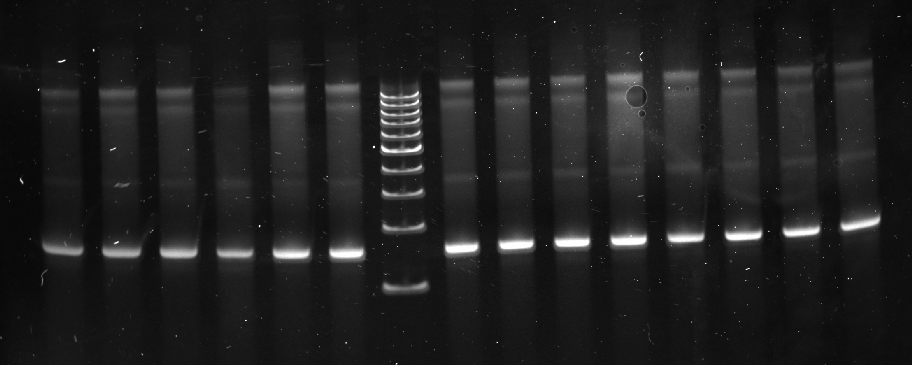
\includegraphics[width=\textwidth]{amplig_a}
    \caption{A}
    \label{fig:amplig_a}
  \end{subfigure}
  \begin{subfigure}[htpb]{0.4\textwidth}
    \centering
    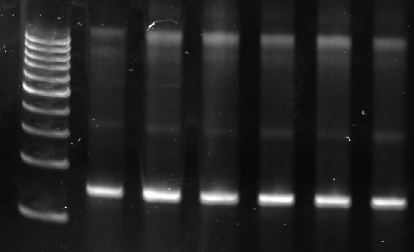
\includegraphics[width=\textwidth]{amplig_b}
    \caption{B}
    \label{fig:amplig_b}
  \end{subfigure}
  \begin{subfigure}[htpb]{0.4\textwidth}
    \centering
    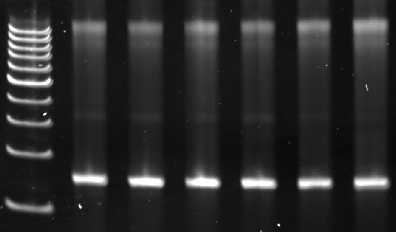
\includegraphics[width=\textwidth]{amplig_c}
    \caption{C}
    \label{fig:amplig_c}
  \end{subfigure}
  \begin{subfigure}[htpb]{0.4\textwidth}
    \centering
    
\includegraphics[width=\textwidth]{test}
    \caption{D}
    \label{fig:amplig_d}
  \end{subfigure}
  \caption{Gel electrophoresis in 8\% TBE gels for (A) amplified lig147 (B) half-C-methylated (C) all-C-methylated, and (D) CpG-methylated DNA. All lanes exhibited a strong band between 100 and 200 nucleotides. Slower-migrating fainter bands corresponded to single-stranded DNA as was expected.}
  \label{fig:amplig}
\end{figure}

\subsection{Nucleosome reconstitution}
\label{ssec:reconstnuc}

EMSA in all cycles yielded strong bands corresponding to naked 147-base pair DNA. It also yielded bands corresponding to reconstituted nucleosomes that are fainter as the proportion of histone octamer decreased in the solution (figure~\ref{fig:reconstnuc}). These observations confirmed that the nucleosome reconstitution protocols based on Dyer (2004) were successful, including for methylated DNA.

\begin{figure}[htpb]
  \centering
  \begin{subfigure}[htpb]{0.4\textwidth}
    \centering
    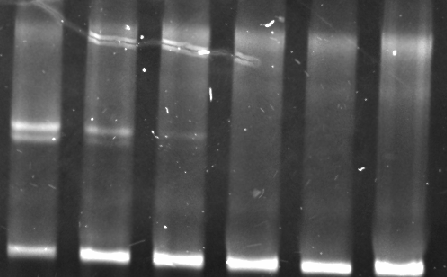
\includegraphics[width=\textwidth]{reconstnuc_a}
    \caption{A}
    \label{fig:reconstnuc_a}
  \end{subfigure}
  \begin{subfigure}[htpb]{0.4\textwidth}
    \centering
    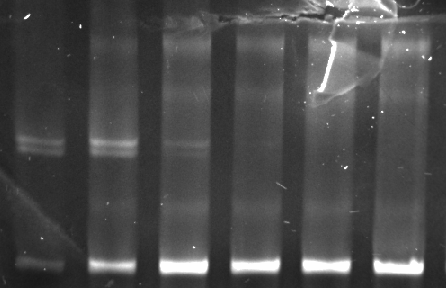
\includegraphics[width=\textwidth]{reconstnuc_b}
    \caption{B}
    \label{fig:reconstnuc_b}
  \end{subfigure}
  \begin{subfigure}[htpb]{0.4\textwidth}
    \centering
    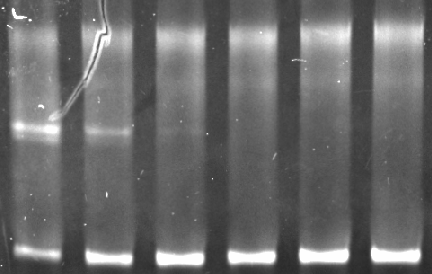
\includegraphics[width=\textwidth]{reconstnuc_c}
    \caption{C}
    \label{fig:reconstnuc_c}
  \end{subfigure}
  \begin{subfigure}[htpb]{0.4\textwidth}
    \centering
    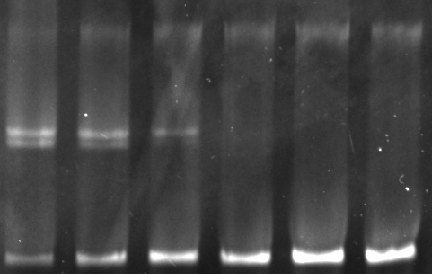
\includegraphics[width=\textwidth]{reconstnuc_d}
    \caption{D}
    \label{fig:reconstnuc_d}
  \end{subfigure}
  \caption{First cycle gel electrophoresis for EMSA in 6\% DNA retardation gels for (A) non-methylated DNA, (B) half-C-methylated (C) all-C-methylated, and (D) CpG-methylated DNA. Lanes for all images (left to right): (1) 1.48:1 histone octamer:DNA, (2) 0.74:1 histone octamer:DNA, (3) 0.37:1 histone octamer:DNA, (4) 0.19:1 histone octamer:DNA, (5) 0.09:1 histone octamer:DNA, and (6) DNA without histone octamer added. These results are representative for all cycles of EMSA SELEX.}
  \label{fig:reconstnuc}
\end{figure}

%% - The sequence preferences of nucleosome 
%% - Disfavored sequences of nucleosome
%% - Methylation effects on nucleosome’s sequence preference

\section{Discussion}
\label{sec:emsaselex_discussion}
%% - The underlying mechanism leading to nucleosome’s sequence preference
%% - Physiological meaning of such preference
%% - Physiological relevance of the methylation effect
%% - A few discussions about Troubleshooting

% I anticipate this to be A LOT shorter

% No quantification of the concentrations of DNA needed here. Focus on sequencing.
Following elution of the DNA from EMSA in the four SELEX cycles, IDT barcodes were added for Illumina sequencing. The DNA elution products from each cycle of EMSA SELEX were used as templates. I tested the use of DreamTaq polymerase and Phusion DNA polymerase (both ThermoFisher) as DNA polymerase enzymes for barcoding.

% Debugging should probably be in a separate subsection in the results or discussion section
Gel electrophoresis of the products amplified by DreamTaq using recommended protocols yielded bands corresponding to 147 base pairs, suggesting that the amplification succeeded (figure~\ref{fig:barcoding_a}). However, gel electrophoresis of the products amplified by Phusion using recommended protocols did not yield this band (figure~\ref{fig:barcoding_b}).

Repeating the Phusion amplification using qPCR yielded saturation curves (figure~\ref{fig:qpcr}), suggesting that amplification indeed took place. As qPCR required a lower concentration of the template, it was hypothesised that Phusion initially failed because the ligand was too concentrated. Different DNA polymerases from different vendors are efficient with differing template concentrations – for example, DreamTaq requires ... while Phusion requires ... (citation needed). Therefore, I diluted the template DNA further by adding \SI{70}{\micro\litre} dilution buffer to each well. The resulting 8\% TBE gel yielded the band corresponding to 147 base pairs (figure~\ref{fig:barcoding_c}), confirming the hypothesis.

\begin{figure}[htpb]
  \centering
  \begin{subfigure}[htpb]{0.4\textwidth}
    \centering
    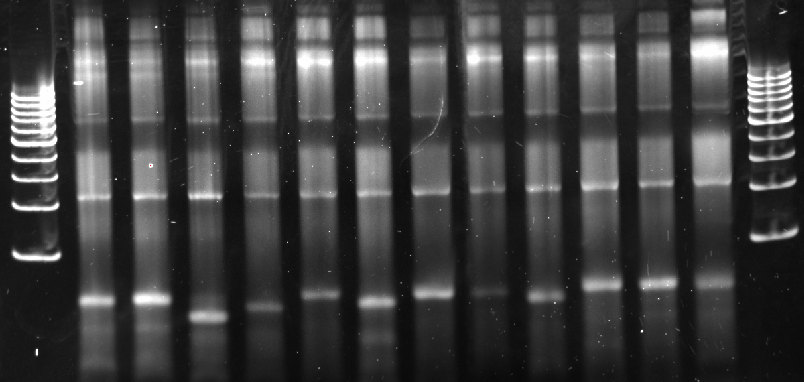
\includegraphics[width=\textwidth]{dreamtaq}
    \caption{A}
    \label{fig:barcoding_a}
  \end{subfigure}
  \begin{subfigure}[htpb]{0.4\textwidth}
    \centering
    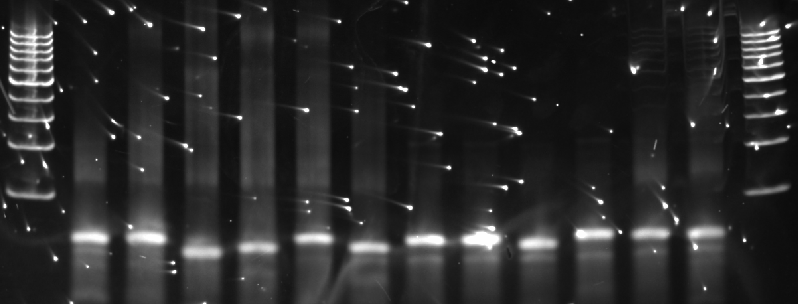
\includegraphics[width=\textwidth]{phusion_old_a}
    \caption{B}
    \label{fig:barcoding_b}
  \end{subfigure}
  \begin{subfigure}[htpb]{0.4\textwidth}
    \centering
    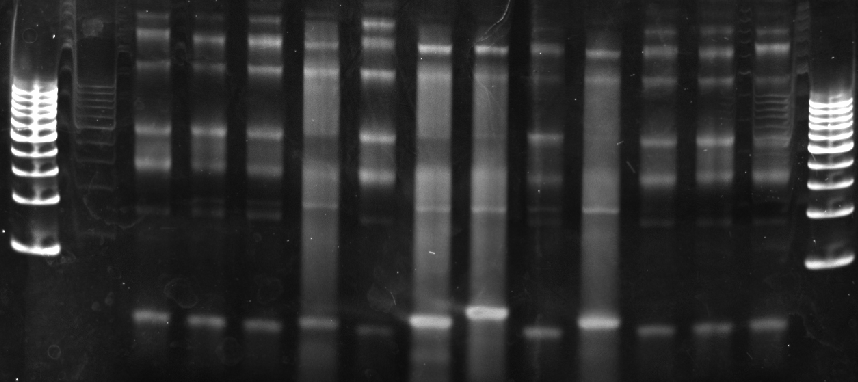
\includegraphics[width=\textwidth]{phusion_new_a}
    \caption{C}
    \label{fig:barcoding_c}
  \end{subfigure}
  \begin{subfigure}[htpb]{0.4\textwidth}
    \centering
    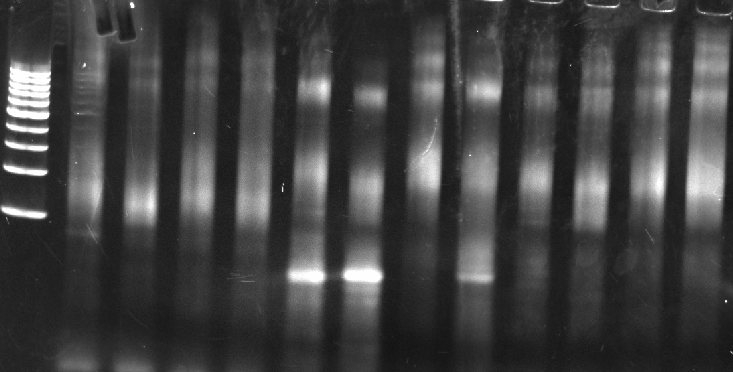
\includegraphics[width=\textwidth]{qpcrgel}
    \caption{D}
    \label{fig:barcoding_d}
  \end{subfigure}
  \caption{A - DreamTaq gel, B - old Phusion gels for rows A and B, C - new Phusion gels for rows A and B, D - qPCR gel}
  \label{fig:barcoding}
\end{figure}

\begin{figure}[htpb]
  \centering
  \begin{subfigure}[htpb]{0.3\textwidth}
    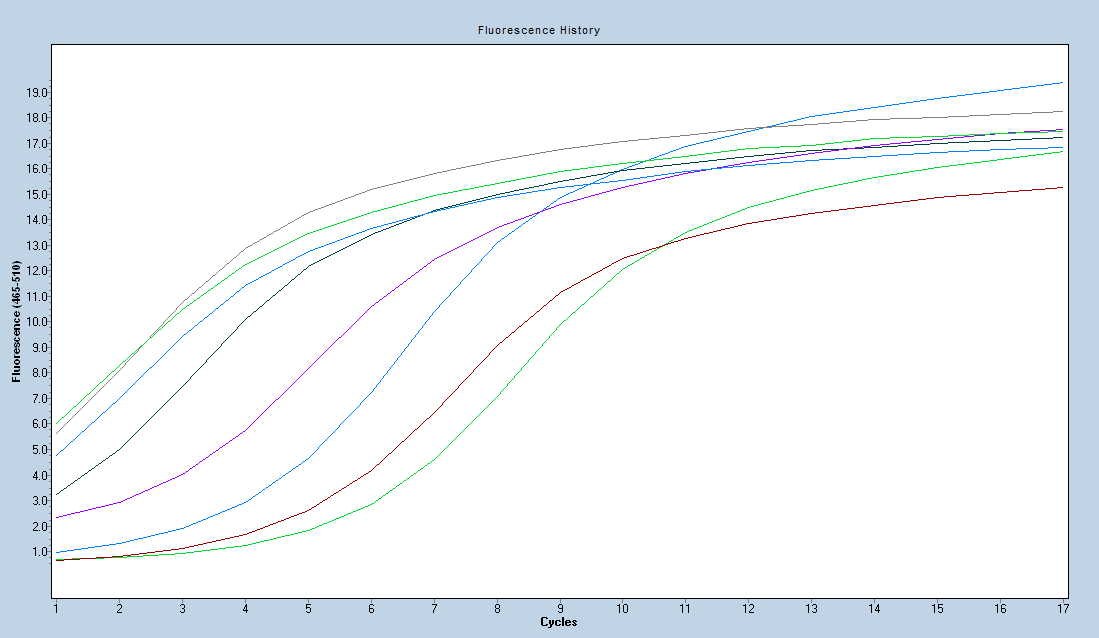
\includegraphics[scale=0.1]{qPCR_B}
    \caption{A}
    \label{fig:qpcr_a}
  \end{subfigure}
  \begin{subfigure}[htpb]{0.3\textwidth}
    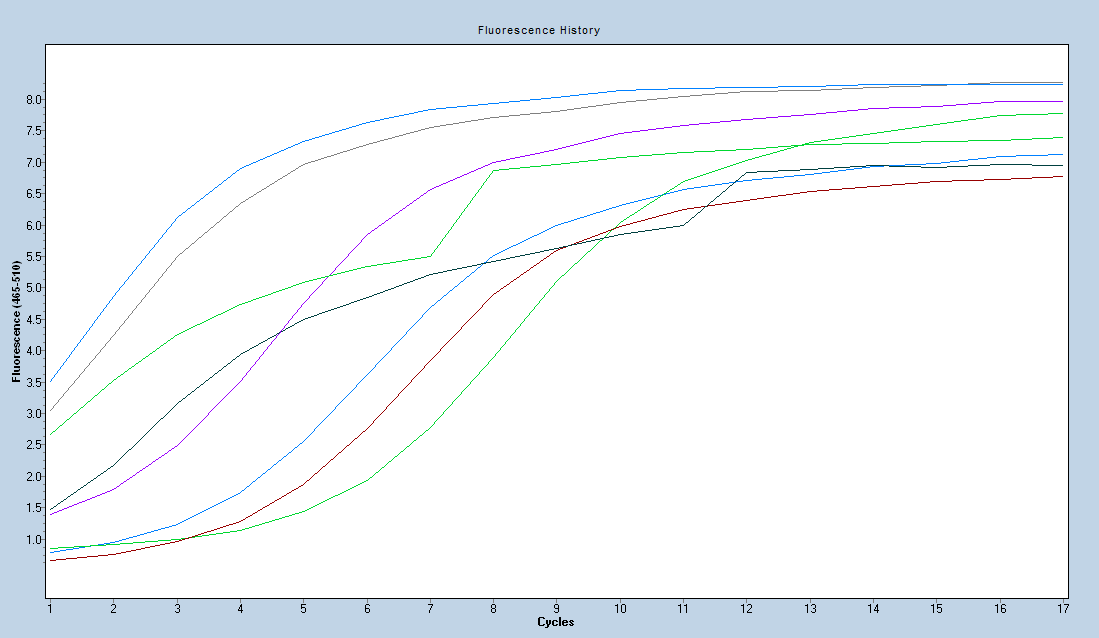
\includegraphics[scale=0.1]{qPCR_D}
    \caption{B}
    \label{fig:qpcr_b}
  \end{subfigure}
  \begin{subfigure}[htpb]{0.3\textwidth}
    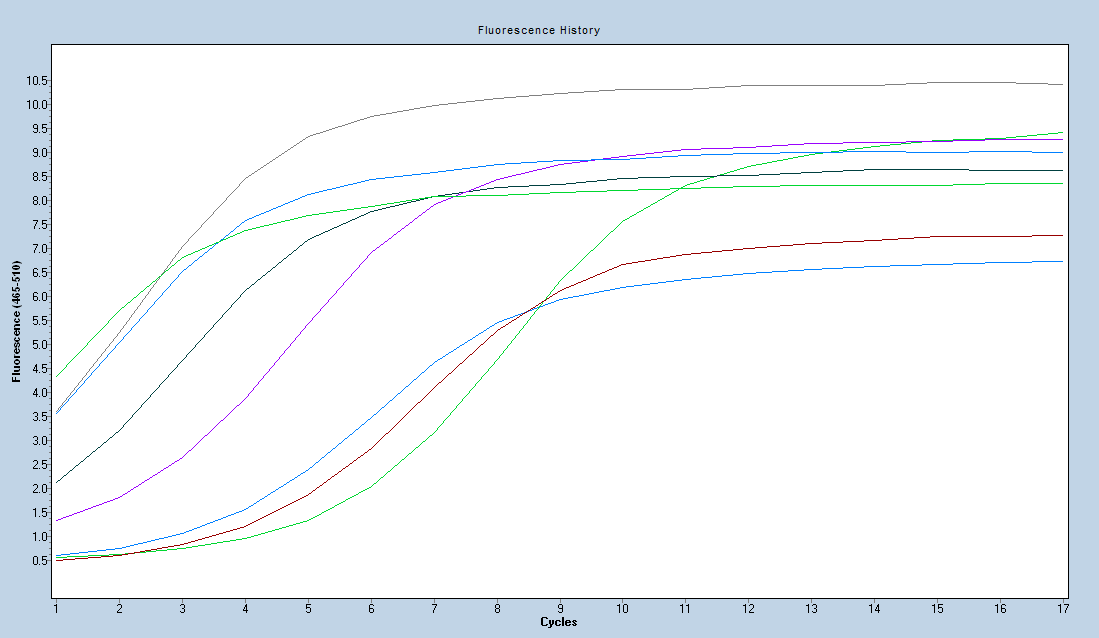
\includegraphics[scale=0.1]{qPCR_F}
    \caption{C}
    \label{fig:qpcr_c}
  \end{subfigure}
  \caption{A - row B, B - row D, C - row H}
  \label{fig:qpcr}
\end{figure}


\chapter{PCR Bias}
\label{ch:pcrbias}

\section{Introduction}
\label{sec:pcrbias_intro}

\subsection{Origin of PCR bias}
\label{ssec:pcrbias_intro_origin}
%% - The origin of PCR bias

\subsection{How PCR bias affects reliability of sequencing results}
\label{ssec:pcrbias_intro_effects}
%% - How PCR bias affects reliability of sequencing results

\subsection{Purpose of study}
\label{ssec:pcrbias_intro_why}
%% - The purpose of this study: provide experiment data, to build a model accounting for such bias, remove such bias in future genomic study

\section{Materials and Methods}
\label{sec:pcrbias_methods}
%% - Most parts are the same as the project 1 [just add references to it??]

The input library was lig147. Pre-mixes for PCR amplification were prepared according to manufacturers' specification for the following DNA polymerases: Phire Hot Start II DNA polymerase (ThermoFisher, F122S), Q5 Hot Start High-Fidelity DNA polymerase (New England BioLabs, M0493S), DreamTaq Hot Start DNA Polymerase (ThermoFisher, EP1701), Pfu Turbo DNA Polymerase (Agilent Technologies, 600250), and Phusion High-Fidelity DNA Polymerase (ThermoFisher, F530L). \SI{25}{\micro\litre} of each pre-mix was mixed with \SI{25}{\micro\litre} of the input library, and amplified by thermocycling according to the protocols specified by the manufacturers of each DNA polymerase.

%% - Data analysis

\section{Results}
\label{sec:pcrbias_results}
%% - Different oligonucleotide bias of different PCR enzymes
%% - The variance caused by bottleneck effect 
%% - Dependency of bias on PCR template concentration
%% - Bias caused by reagents from different company
%% - Bias from PCR Purification

\section{Discussion}
\label{sec:pcrbias_discussion}
%% - Relevance of such bias to previous sequencing data
%% - Hints to data analysis in the future 
%% - A few discussions about Troubleshooting

\chapter{Acknowledgements}
\label{ch:ack}

Acknowledgements.

\printbibliography

\end{document}
